\chapter{Introduzione}\label{introduzione}

La laringoscopia è una procedura medica utilizzata per ispezionare la laringe e per diagnosticare, ed eventualmente curare, i disturbi della laringe e delle corde vocali.

In particolare ci sono due tipi di laringoscopia, quella indiretta e quella diretta. La prima fa uso di un semplice specchio e di una fonte luminosa, la seconda richiede l'uso di un laringoscopio e una anestesia.

Il laringoscopo è uno strumenti che grazie a una fibra ottica, una sorgente luminosa e una telecamera permette di osservare nei minimi dettagli la laringe e tutti gli elementi che la costituiscono come le epiglottide e le corde vocali\cite{giorgio_cenni_2008}. In particolare permette di aiutare a diagnosticare malattie come la laryngeal squamous cell carcinoma (SCC), la cui diagnosi precoce riduce la mortalità del paziente\cite{moccia_larynge}.

L'obiettivo di questa tesi è quello di usare l'uso di algoritmi di apprendimento automatico basati sul transfer learning e sul  preprocessing di immagini  per la classificazione dei frame di una laringoscopia, in particolare la selezione degli informative-frame e lo scarto di tutti i frame non utili come frame pieni di saliva o non a fuoco. In \cref{fig:larynges} alcuni esempi di frame da tenere estratti da una laringoscopia.

\begin{figure}[ht]
    \centering
    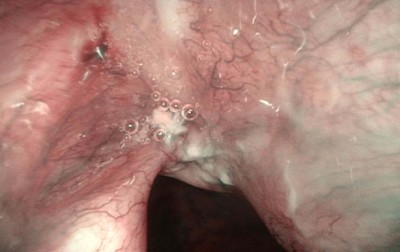
\includegraphics[width=0.3\textwidth]{introduzione/Larynge-1.jpg}
    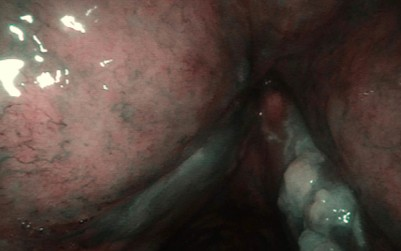
\includegraphics[width=0.3\textwidth]{introduzione/Larynge-2.jpg}

    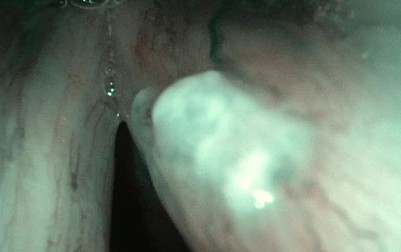
\includegraphics[width=0.3\textwidth]
    {introduzione/Larynge-3.jpg}
    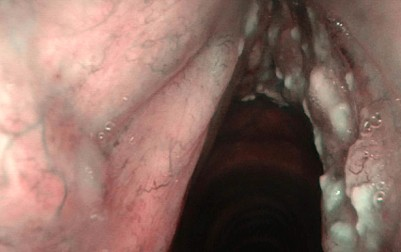
\includegraphics[width=0.3\textwidth]{introduzione/Larynge-4.jpg}
    \caption{Esempio di fotogrammi endoscopici laringei}
    \label{fig:larynges}
\end{figure}

\section{Descrizione dei dataset}\label{descrizione-dei-dataset}
